%
%  
%  
%
%%%%%%%%%%%%%%%%%%%%%%%%%%%%%%%%%%%%%%%%%%%%%%%%%%%%%%%%%%%%%%%%%%%%%%%%%%%%%%%%%%%%%%%%%%%%%%%%%%%%%%%%%%%%%%%%%%%%%%%%%%%%%%%%%%%%%%%%%%%%%%%
\documentclass[10pt, onecolumn]{witseiepaper}


\usepackage{KJN}
\usepackage{graphicx}
\usepackage{rotating}
\usepackage{float}
\usepackage{pdfpages}
\usepackage{listings}
\usepackage{color}

\definecolor{codegreen}{rgb}{0, 0.6, 0}
\definecolor{codegray}{rgb}{0.5, 0.5, 0.5}
\definecolor{codepurple}{rgb}{0.58, 0, 0.82}
\definecolor{backcolour}{rgb}{0.95, 0.95, 0.92}

\graphicspath{{Images/}}
%%%%%%%%%%%%%%%%%%%%%%%%%%%%%%%%%%%%%%%%%%%%%%%%%%%%%%%%%%%%%%%%%%%%%%%%%%%%%%%%%%%%%%%%%%%%%%%%%%%%%%%%%%%%%%%%%%%%%%%%%%%%%%%%%%%%%%%%%%%%%%%
\ifpdf
\pdfinfo {
/Title ()
/Author ()
/CreationDate (D:201604201500)
/ModDate (D:201604201500)
/Subject (ELEN7045 - )
/Keywords ()
}
\fi
\pagestyle{plain}

%%%%%%%%%%%%%%%%%%%%%%%%%%%%%%%%%%%%%%%%%%%%%%%%%%%%%%%%%%%%%%%%%%%%%%%%%%%%%%%%%%%%%%%%%%%%%%%%%%%%%%%%%%%%%%%%%%%%%%%%%%%%%%%%%%%%%%%%%%%%%%%
\begin{document}

\begin{titlepage}
	
	\newcommand{\HRule}{\rule{\linewidth}{0.5mm}} 
	
	% Defines a new command for the horizontal lines, change thickness here
	\begin{center}
		
		% Center everythingn the page
		\textsc{\LARGE ELEN7045}\\[0.5cm]
		
		% Name of your university/college
		\textsc{\Large University of Witwatersrand}\\[0.25cm]
		
		% Major heading such as course name
		\textsc{\large SD Methodologies, Analysis and Design}\\[0.5cm]
		
		% Minor heading such as course title
		\HRule \\[0.4cm]
		{ \huge \bfseries Assignment 2 : Dynamic Proxies}\\[0.25cm]
		
		% Title of your document
		\HRule \\[1.25cm]
		\begin{minipage}
			{0.4
				\textwidth} 
			\begin{flushleft}
				\large \emph{\textbf{Authors:}}\\
				Francois  \textsc{van Niekerk} \\
			\end{flushleft}
		\end{minipage}
		~ 
		\begin{minipage}
			{0.4
				\textwidth} 
			\begin{flushright}
				\large \emph{\textbf{Student Number:}} \\
				1234567  \\
			\end{flushright}
		\end{minipage}
		
		\begin{minipage}
			{1	\textwidth} 
			\begin{flushright}
				\center\large{\textit{\\This is a declaration that the following student authored this report.}} \\
			\end{flushright}
		\end{minipage}\\[2cm]
		
	%	\begin{figure}[H]
	%		\center{\includegraphics[width=.25\linewidth]{WITSimage}} 
	%	\end{figure}
				
		{\large \today}\\[1.25cm]
				
					
		 \begin{minipage}
		 	{1	\textwidth} 
		 	\begin{flushleft}
		 	
		 	\large \emph{\textbf{Abstract:}}\\
		  			 			 	
		  	\end{flushleft}
		 \end{minipage}
	\end{center}

\end{titlepage}	
	

\tableofcontents
%\newpage

%\listoffigures
%\listoftables
%\newpage

%%%%%%%%%%%%%%%%%%%%%%%%%%%%%%%%%%%%%%%%%%%%%%%%%%%%%%%%%%%%%%%%%%%%%%%%%%%%%%%%%%%%%%%%%%%%%%%%%%%%%%%%%%%%%%%%%%%%%%%%%%%%%%%%%%%%%%%%%%%%%%%
\section{INTRODUCTION}

intro blah blah \cite{Java}


%%%%%%%%%%%%%%%%%%%%%%%%%%%%%%%%%%%%%%%%%%%%%%%%%%%%%%%%%%%%%%%%%%%%%%%%%%%%%%%%%%%%%%%%%%%%%%%%%%%%%%%%%%%%%%%%%%%%%%%%%%%%%%%%%%%%%%%%%%%%%%%

\section{Definition of Dynamic Proxies}

\begin{figure}[h]
	\centering
	\fbox{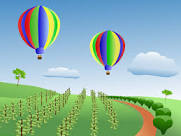
\includegraphics[scale=0.5]{sample}}
	\caption{Sample Caption}
	\label{SampleLabel}
\end{figure}

\section{Code Listings on how to create a dynamic proxy}

\section{Dynamic proxies in Java and C\#}


%\subsection{Application Planning}

\section{A discussion of the features of Object-Oriented Programming dynamic proxies rely on, and the constraints involved when using dynamic proxies}

\section{Conclusion}


\newpage

\bibliographystyle{witseie}
\bibliography{bibliography}
\end{document}
